\documentclass[11pt,a4paper]{report}

\usepackage[utf8]{inputenc}
\usepackage[T1]{fontenc}
\usepackage[english]{babel}
\usepackage[top=2cm,bottom=2cm,left=2cm,right=2cm]{geometry}
%\usepackage{url}
%\usepackage{fancyhdr}
\usepackage{sectsty}
\usepackage{wrapfig}
\usepackage{titlesec}
\usepackage{setspace}
\usepackage{graphicx}
\usepackage{lmodern}
\usepackage{url}
\usepackage{amsmath}
\usepackage{amssymb}
\usepackage{mathrsfs}
\usepackage{fancyhdr}
\usepackage{gensymb}
\usepackage{enumerate}
\usepackage{hyperref} % Créer des liens et des signets 
\usepackage[cc]{titlepic}
\usepackage{caption}
\usepackage{verbatim}
\usepackage{color}
\usepackage{subfigure}
\usepackage{epsfig}
\usepackage{amsmath}
\usepackage{cancel}
\usepackage{enumitem}
\usepackage[justification=centering]{caption}

\setlist[enumerate]{font=\bfseries}


\title{
\rule{15cm}{1pt} \\
\Large {\bfseries Intelligent mobile robotics} \\
\Large {\bfseries Assignment 2}\\
\rule{15cm}{1pt}}
\author{Sami Sellami}	

\titlepic{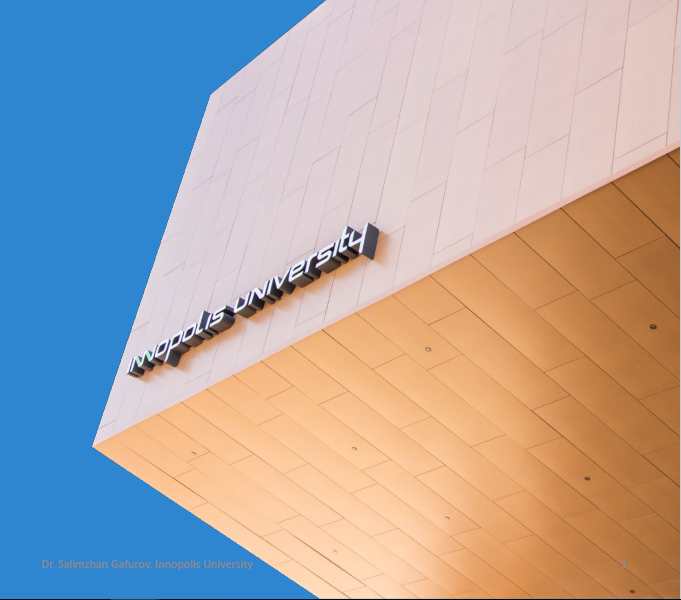
\includegraphics[width=10cm]{Innopolis_image.PNG}} 
\date{\today}
 
\begin{document}
\pagenumbering{arabic}
\setcounter{page}{1}
\setcounter{secnumdepth}{1}
	
\fontfamily{ptm}\selectfont

\maketitle

\titlelabel{\thetitle)\quad}
\titlespacing{\chapter}{0cm}{0cm}{0cm}
\titlespacing{\section}{0.2cm}{0cm}{0cm}

\subsection{\textbf{Problem1:}}

The task is related to line extraction, we have radar data form the scanning of a room (room 303 in the university ) and we need to extract the line in the point cloud using different methods, namely; split and merge, line regression and hough transform
 
 \textbf{split and merge}:
This is a popular algorithm which uses recursive procedure of fitting and splitting, in our case we used the so called Iterative end point fit which simply connects the end points for line fitting, the splitting is done until the distance from the line to the farthest point is less than a predifined threshold, at the end we used the information of slopes to merge the line that are colinear enough (wrt a specific threshod) \\
Figure \ref{fig1} show the result of the line fitting:

\begin{center}\label{fig1}
	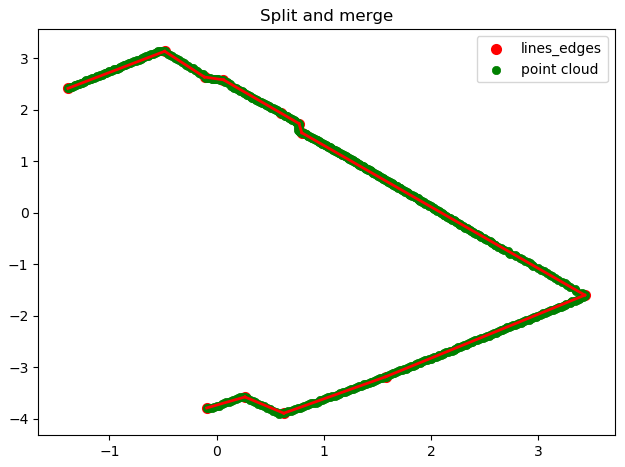
\includegraphics[width=8cm]{Capture1.png}
	\captionof{figure}{ {\small Split and merge line fitting}}	
\end{center}

\textbf{line regression}:
Line regression uses a sliding windows of size $N_{f}$, when the windows is sliding, a line is fitted to the points inside the window using least square method , also a fidelity array is computed wich contains the mahalalobis distance between the last two windows, when all the points have been analized, we merge the lines that have similarities in the fidelity array, meaning that  distance between them is not too high \\
Figure \ref{fig2} show the result of the procedure

\begin{center}\label{fig2}
	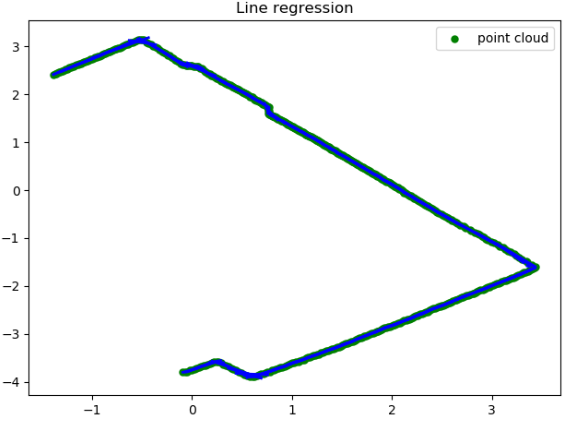
\includegraphics[width=8cm]{Capture2.png}
	\captionof{figure}{ {\small Line regression}}	
\end{center}

\textbf{Hough transform}:
Hough transfom maps image space into hough space it uses the proporty that a line in image space is a point in the hough space, OpenCV provide a function to compute the hough transform of an image (\textbf{\textit{cv2.HoughLines}} ), to uses the funciton, we needed to transform our point cloud into a matrix corresponding to an image.
The result is show in the following image 


\begin{center}\label{fig3}
	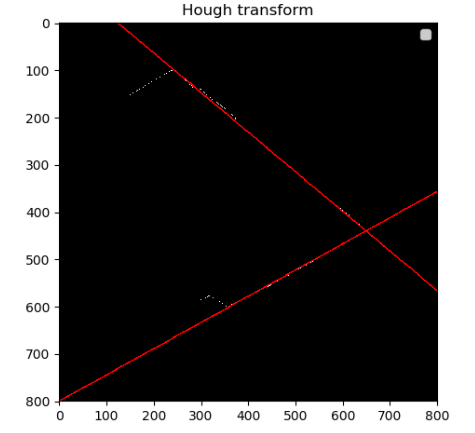
\includegraphics[width=8cm]{Capture3.png}
	\captionof{figure}{ {\small Hough transform}}	
\end{center}

\textbf{Checking the time exectution}:
The next diagram shows the time execution of each algorithm, we can see that line regression takes much time to compute, this is due to the fact that its  two step algorithm and the computations are higher


\begin{center}\label{fig4}
	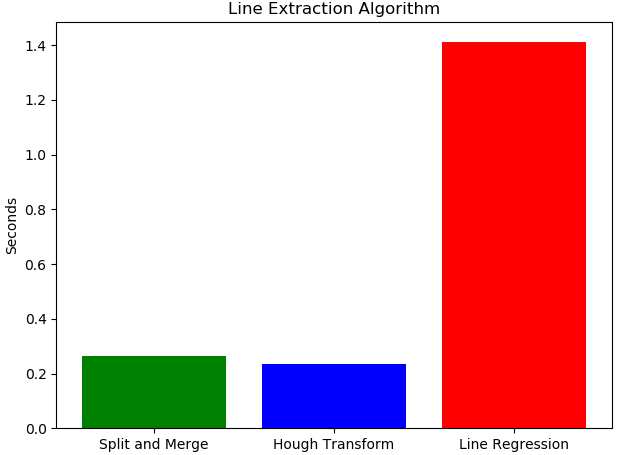
\includegraphics[width=8cm]{Capture4.png}
	\captionof{figure}{ {\small Time of execution}}	
\end{center}

\subsection{\textbf{Problem2:}}
The task is to use \textbf{SIFT} feature desctiptor to detect and match features between five successive images, for this we located a bouding box around our object of interest (car moving in the driveway) and then we used OpenCV library to detect the keypoints in the box, the image below shows the result;

\begin{center}\label{fig5}
	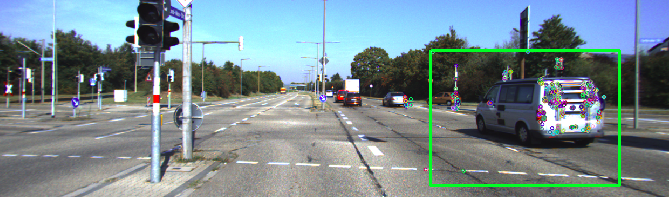
\includegraphics[width=12cm]{Capture5.png}
	\captionof{figure}{ {\small Keypoints detection}}	
\end{center}

After that we implemented our feature descriptor which consist of of a 128 vector array of the histogram of orentation in 8 directions of the neighbouring region, the correspondance between the keypoints detected in two successive images is shown below:


\begin{center}\label{fig6}
	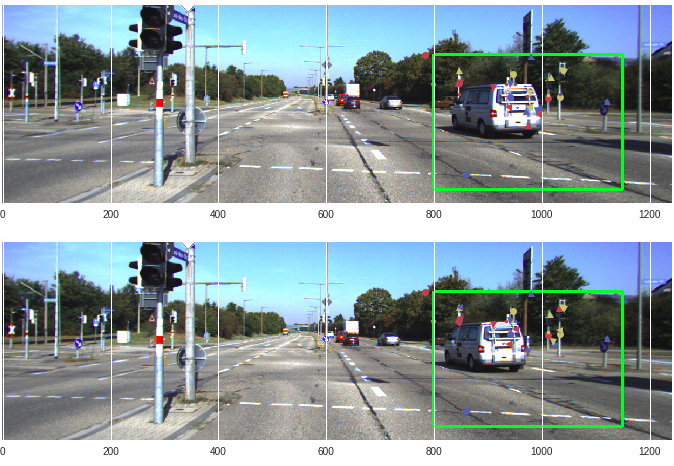
\includegraphics[width=12cm]{Capture6.png}
	\captionof{figure}{ {\small Keypoints detection and matching}}	
\end{center}
 
  
\end{document}	
